\chapter{METODOLOGI}

\section{Tahap Pelaksanaan Studi}
Metodologi berisi penjelasan untuk mengartikulasikan rencana penelitan/perancangan dengan cukup jelas dan detil. Metodologi penelitian/perancangan/pembangunan alat memiliki banyak dimensi dan metode penelitian/perancangan/pembangunan alat merupakan bagian dari metodologi penelitian/perancangan/pembangunan alat. Salah satu contoh metodologi penelitian dapat dilihat pada Gambar \ref{fig:diagram}.

\begin{figure}[h!]
    \centering
    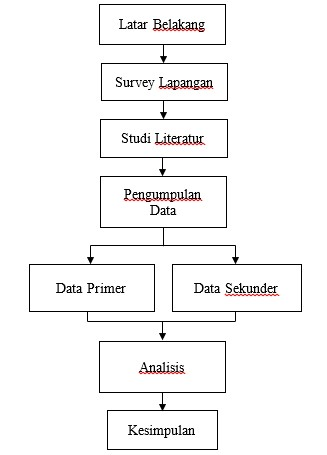
\includegraphics[width=0.6\textwidth]{gambar/diagram.jpg}
    \caption{Diagram Alir Penelitian}
    \label{fig:diagram}
\end{figure}

\section{Data Penelitian}
Data penelitian adalah informasi yang dikumpulkan, diukur, dan dianalisis selama proses penelitian. Data ini digunakan untuk menjawab pertanyaan penelitian, menguji hipotesis, atau membangun teori. Data penelitian yang digunakan berupa data primer maupun data sekunder Contoh data penelitian sekunder dapat dilihat pada Lampiran 1.

\section{...} % disesuaikan dengan metodologi yang digunakan

\section{...} % disesuaikan dengan metodologi yang digunakan

\section{Jadwal Pelaksanaan TA}
\definecolor{ITSBlue}{RGB}{0,114,198}
\renewcommand{\arraystretch}{1.3} % spasi antar baris
\setlength{\tabcolsep}{4pt}       % spasi antar kolom

\begin{tabularx}{\textwidth}{|p{4cm}|*{6}{>{\centering\arraybackslash}X|}}
\hline
\textbf{Kegiatan} & \multicolumn{6}{c|}{\textbf{Bulan}} \\ 
\cline{2-7}
 & 1 & 2 & 3 & 4 & 5 & 6 \\ \hline
Studi Literatur     & \cellcolor{ITSBlue} & \cellcolor{ITSBlue} &   &   &   &   \\ \hline
Perancangan Alat    &   & \cellcolor{ITSBlue} & \cellcolor{ITSBlue} &   &   &   \\ \hline
Pengujian           &   &   &   & \cellcolor{ITSBlue} & \cellcolor{ITSBlue} &   \\ \hline
Analisis Data       &   &   &   &   & \cellcolor{ITSBlue} & \cellcolor{ITSBlue} \\ \hline
Penyusunan Laporan  &   &   &   &   &   & \cellcolor{ITSBlue} \\ \hline
\end{tabularx}